\chapter{OpenCL heterogenous programming platform}
This chapter will describe OpenCL. A framework for writing applications that
harness computational capabilities of heterogeneous hardware environment on
which applications are run. Since the introduction of programmable pipeline
in GPUs\footnote{Graphics Processing Unit} an opportunity appeared to use
capabilities of these devices to offload highly parallel, computationally
intensive tasks from main CPU\footnote{Central Processing Unit}. OpenCL can also
expose dedicated hardware units designed to perform certain specialized tasks
like Digital Signal Processing.

OpenCL is used in programming project described in \autoref{chap:project}.
Metaballs and Marching Cubes algorithm are implemented with it. Marching Cubes
algorithm and its OpenCL implementation are described in detail in
\autoref{chap:marchingcubes}.

\section{Introduction}
This section is based on \cite{Kirk:2010:PMP:1841511} and
\cite{gaster2012heterogeneous}.

\subsection{Beginnings of programmable GPUs}

From early 1980s to late 1990s most graphic hardware was fixed--function.
I.e. dedicated graphics units exposed fixed set of functions that were
implemented in hardware or drivers. It wasn't possible to write custom program
that would be executed on the GPU.

As the complexity of fixed--function APIs expanded, hardware vendors implemented
them with general purpose processors that could run some limited instruction set
on many processors. This instruction set was used to implement graphics APIs
like OpenGL or DirectX.

In 2001 NVIDIA released GeForce 3 graphics card that exposed this internal
instruction set to users of OpenGL and DirectX APIs. ATI technologies followed
with Radeon 9700 that could also run programs supplied by the user on the GPU.
DirectX 8 and OpenGL introduced programmable vertex stage. With
DirectX 9 another programmable stage was introduced, the pixel (or fragment in
OpenGL terminology) shader. At this point, vertex and pixel shaders were
implemented via separate chips in the GPU. In 2005, with release of XBox 360
first unified architecture was introduced, on which vertex and fragment shaders
were run on the same processor.

Graphics processing, that these devices were build for is very well suited for
parallelization. Vertex shader stage takes list of vertices as its input and
maps them onto the screen optionally defining colour of the vertex. Each
vertex is processed independently making it possible to process many vertices
at the same time.

Pixel shader stage receives position of the point and returns final colour of
the pixel. This also is done independently for each pixel.

\subsubsection[Early attempts at GPGPU]{Early attempts at GPGPU\footnote{General Purpose GPU}}

With the unification of computational resources in the GPUs they started to
resemble highly parallel computers. Researchers noted this fact, and tried to
harness enormous parallel performance for workloads other than graphics.

GPUs of DirectX 9 era were still designed in graphics processing in mind.
Although there were programmable stages in the pipeline, types of input and
output parameters in each stage were severely limited. Moreover, the final
result was generated as a pixel buffer, so the programmer had to map outputs of
his algorithm to 2D screen space with pixel colour as output. Inputs to the
pixel shader stage had to be supplied by textures.

Even with these issues, researchers who managed to port their algorithms to
GPUs reported great performance benefits.

\subsubsection{CUDA}

When working on Tesla GPU architecture, engineers at NVIDIA realized the
potential in providing device's resources in easier way. Additional instructions
and functionalities were added to the device. Among them, read and write
operation with arbitrary offsets\footnote{Shaders could only write to predestined
places in memory, reserved for pixel output}, synchronization barriers for
groups of threads, atomic read/write operations. New parallel programming model
was developed that defined hierarchy of threads.

To expose all these features to programmers new C--like language was
created and named CUDA\footnote{Compute Unified Device Architecture}.

CUDA is capable of operating without any DirectX or OpenGL context. Device it's
run on doesn't even have to be connected to any display output. CUDA programs
are usually inlined in larger C or C++ programs and are called \emph{kernels}.
Special compiler called \emph{nvcc} is used to compile kernel code. For more
information about CUDA refer to official CUDA website\footnote{\url{http://www.nvidia.com/object/cuda_home_new.html}}.

\subsubsection{Inception of OpenCL}

On June 16th, 2008 Khronos Group announced formation of Compute Working Group (CWG)
that was tasked with establishing open standard for programming heterogeneous
CPU and GPU environments\footnote{\url{https://www.khronos.org/news/press/khronos\_launches\_heterogeneous\_computing\_initiative}}.
CWG consisted of many hardware and software vendors interested in
standardization of such API.

Compute Working Group adopted proposal of Apple Inc. that submitted programming
interface called Open Compute Language (OpenCL). Apple was already developing
OpenCL for quite some time to have it ready for its upcoming Mac OS X Snow
Leopard release.

On December 9th, 2008 final specification of OpenCL 1.0 was
released\footnote{\url{https://www.khronos.org/news/press/the\_khronos\_group\_releases\_opencl\_1.0\_specification}}.
Releases of conforming implementations from hardware vendors followed\footnote{\url{http://www.khronos.org/conformance/adopters/conformant-products/\#opencl}}.

\subsection{Specification}
OpenCL specification is maintained by the Khronos Group. It consists of C API
and Kernel language that is similar to C99. Khronos releases official C++
wrapper API\footnote{This wrapper API is used in programming project of this thesis}.

Unofficial bindings for various languages and frameworks also exist. Among others
\begin{itemize}
	\item PyOpencl\footnote{\url{http://mathema.tician.de/software/pyopencl}}
		for Python
	\item JOCL\footnote{\url{http://www.jocl.org/}} for Java.
	\item fortrancl\footnote{\url{http://code.google.com/p/fortrancl/}} for Fortran
	\item gocl\footnote{\url{https://github.com/elima/gocl}} wrapper for C
		applications based on GObject
	\item QtOpenCL\footnote{\url{http://doc.qt.digia.com/opencl-snapshot/index.html}}
		wrapper based on Qt library semantics.
\end{itemize}

\section{Logical abstraction of computational resources}
\label{sec:cllogicalabstraction}
OpenCL aims to be API that lets hardware manufacturers expose various kinds of
devices to the programmers in a consistent and abstracted way. To fulfil this
requirement OpenGL defines logical hierarchy of computational resources.
Hardware vendors map real hardware to this abstraction in their implementations
of OpenCL.

OpenCL defines one processor (\emph{host}) that is coordinating execution of
OpenCL kernels on one or more \emph{devices}. Host, is executing functions from
C API portion of the specification. It's responsible for discovering available
devices, setting up contexts for them, allocating memory on host and devices,
queuing execution of kernels and initiating transfer of data between various
memories.

Diagram of this logical structure is presented in \autoref{fig:clhw}.

\begin{figure}[h]
	\begin{center}
		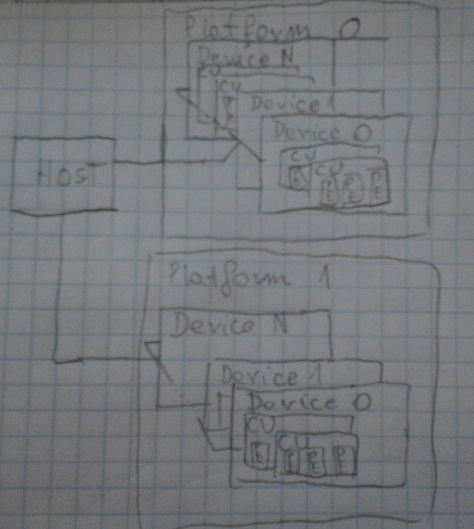
\includegraphics[scale=0.7]{chapters/opencl/opencl_hwmodel.jpg}
	\end{center}
	\caption{Logical partitioning of hardware in OpenCL}
	\label{fig:clhw}
\end{figure}

\subsection{Platforms}

On the top of the hierarchy is \emph{Platform}. It is usually an implementation
of OpenCL by a single vendor. To query list of available platform in the system
function \texttt{clGetPlatformIds()} must be called twice. Once with parameter
\texttt{platforms} set to \texttt{NULL} to obtain number of platforms, and
second time, with \texttt{platform} parameter set to array that will fit
number of \texttt{cl\_platform\_id} structures equal or greater than the number
in argument \texttt{num\_platforms} retrieved on first invocation of this
function.

Note however, that OpenCL is usually loaded as a dynamic library provided by
vendor. These libraries will usually return only one platform.

To address this problem Khronos Group introduced \texttt{cl\_khr\_icd} extension
that depending on operating system, will look for list of installed OpenCL
ICDs or Installable Client Drivers in place specific for given OS. If
implementation supports this extension, new function \texttt{clIcdGetPlatformIDsKHR}
is available that will present to the user platforms from all vendors available
on the system. This extension also makes sure, that function calls with OpenCL
object created in certain platform will be routed to implementations in this
platform.

\subsection{Devices}

Platform, may contain one or more \emph{devices}. Devices are units that
actually execute the kernel code. Device may map for example to single GPU or
CPU.

For example, NVIDIA OpenCL implementation presents each GPU available in the
system as separate device. OpenCL from AMD besides presenting GPUs also presents
supported CPUs as devices.

Device is last entity in hierarchy that has its distinct API object. Further
elements cannot be operated on, and are just abstract concepts to which vendors
map their hardware.

These elements are \emph{compute units} which are comprised of \emph{processing
elements}. Devices can be queried for number of compute units they contain
through \texttt{clGetDeviceInfo()} function.


Exact details of mapping is dependant on OpenCL vendor. Underlying architectures
of GPUs, CPUs and DSPs\footnote{Digital Singal Processors} can differ greatly
even within the same class of devices.

Specifics of implementation on selected devices supporting OpenCL will be
presented in \autoref{sec:climpl}.

\section{Memory model}

\begin{figure}[htpb]
  \begin{center}
    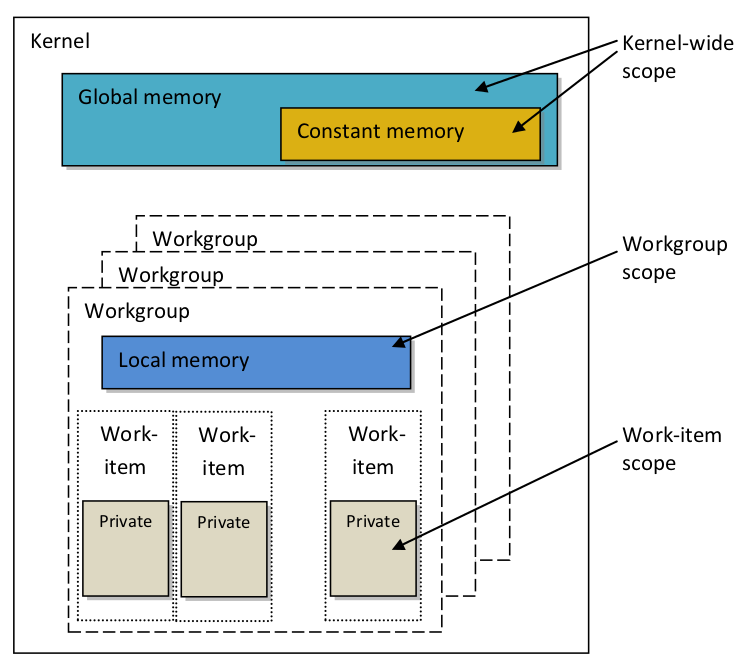
\includegraphics[width=\textwidth]{chapters/opencl/memory.png}
  \end{center}
  \caption{Abstract memory model of OpenCL \parencite{gaster2012heterogeneous}}
  \label{fig:clmemmodel}
\end{figure}\todo{replace \autoref{fig:clmemmodel} with TikZ graphic}

OpenCL provides layer of abstraction on device memory. Depending on the
capabilities of given device, some of memories described below may be
unavailable.

Below are descriptions of memories defined by OpenCL specification. They are
divided to Host-side and Device-side memories.

\subsection{Host-side memory model}

This is the model from the perspective of code that runs on the host. The one
that executes OpenCL library functions. Three types of memory are distinguishable
in this context:

\begin{description}
  \item[Host memory]
    memory that is allocated by the host code with standard allocation techniques
    like \texttt{malloc()}. It's not managed by OpenCL runtime.
  \item[Buffers]
    objects that are handles for global or constant memory allocated on host.
    Buffers are similar in nature to flat C arrays. They have linear addressing,
    so pointer arithmetic is possible in kernel code.

    Buffers differ however in one one crucial point with host memory. Operations
    on them are asynchronous. Functions like \texttt{clEnqueue\-Read\-Buffer()} that
    transfer data between host and device return immediately, and the transfer
    starts in the background. Event mechanism may be used for synchronization
    (see \autoref{sub:clevents}).
  \item[Images]
    Images are somewhat similar to buffers, but differ in fundamental way.
    Unlike buffers, images can be multidimensional. They are not laid flatly in
    memory, but in a way that preserves spatial locality of points within the
    image\footnote{For example by Z-order mapping \parencite{gaster2012heterogeneous}},
    so they cannot be adressed directly but through sampling object, that define
    access patterns to images. They are also limited in terms of supported
    datatypes to ones that are relevant in graphics; no arbitrary structures can
    be held in images.

    Images are abstraction of texturing units available in GPU shaders. Because
    of this heritage, images are not supported on every OpenCL implementation.

\end{description}
\todo{If time allows, write about pinned memory}

\subsection{Device-side memory model}

These are memories, as seen by kernels.

\begin{description}
  \item[Global memory]
    kernel-wide memory that is visible to all compute units on the device.
    It is the only memory that can be used for transferring data between host and
    device. This is also usually slowest type of memory on the device by raw
    throughput.
  \item[Constant memory]
    memory designated for data that is going to be accessed simultaneously by
    many threads. Its contents cannot change throughout the lifetime of the
    kernel. If available it's usually implemented with specialized hardware
    and/or caching strategies.
  \item[Local memory]
    Special memory area that resembles software-controlled cache. This area is
    valid only within a single workgroup (see \autoref{subsub:clworkgroups}). It's
    expected to be much faster than global memory\footnote{However it's not guaranteed},
    so it can be used as a scratchpad area for threads in one workgroup.

    It may be implemented e.g. as separate chip in Compute Unit.

    Local memory can be declared for workgroup in two ways, either dynamically,
    by setting kernel parameter prefixed with \texttt{\_\_local} to NULL with
    desired size parameter, or statically as an array in kernel with the same
    prefix.

  \item[Private memory]
    valid within a single thread. Every non-prefixed variable and all function
    arguments that are not pointers land in this memory. It may be implemented
    with registers\footnote{GPUs, usually don't have stack, so every variable
    is stored in very limited number of registers}. If number of registers is
    exceeded, they may be spilled to global memory, what can have very
    detrimental impact on performance. Number of registers used by kernel must
    be thus carefully controlled.

    Private memory is the fastest available type of memory. For GPUs it's usually
    orders of magnitude faster than global or local memory.
\end{description}

\section{Execution model}
\label{sec:clexecmodel}

This section will describe OpenCL object that mange execution of programs on the
device and stages of such execution.

\subsection{Context}

Context is a structure that coordinates communication between host and devices
and keeps information about memory objects. 

It is created by providing list of devices to \texttt{clCreateContext()}
function. Devices must all come from the same platform, as returned by
\texttt{clGetDeviceIDs()}. There is a convenience function \texttt{clCreateContexFromType()}
that creates context from all devices of given type from one platform \parencite{openclspec}.

\subsection{Programs and Kernels}

To execute kernel code on the device, it must be first provided to specialized
compiler that tranlates human--readable instructions to machine--specific code.

Kernel code must be fed to \texttt{clCreate\-Program\-WithSource()} function in the form of
pointer to character array. OpenCL implementation takes this textual
representation and translates in runtime. It's worth noting, that OpenCL kernel
code is provided to the library in source form. This may be not suitable for
secret proprietary algorithms. For this reason, with OpenCL 2.0 Provisional
specification Khronos released specification for common intermediate
representation called SPIR\footnote{Standard Portable Intermediate Representation
  \url{http://www.khronos.org/registry/cl/specs/spir_spec-1.2-provisional.pdf}}.

There is another function that creates program objects named\\
\texttt{clCreate\-Program\-With\-Binary()} that takes binary representation of OpenCL
code. This function however, is highly device--specific. It can only be used
for caching compiled programs the first time application is run so no compilation
is needed during subsequent runs.

After creating program object, it isn't yet compiled. Compilation is triggered
by \texttt{cl\-Build\-Program()} function.

One program object may have been compiled from a source string containing many
OpenCL kernels. Each function prefixed with \texttt{\_\_kernel} in such string
may be used to create separate kernel with \texttt{clCreateKernel()} function by
providing build program object and kernel function name, or with
\texttt{clCreateKernelsInProgram()} function that creates kernel objects from
all kernel functions present in program object.

\subsubsection{Supplying arguments to kernels}

Since kernels aren't normal host function, they aren't invoked as such. Because
of that, arguments for kernels must be supplied in specific way. Each argument
must be set with separate call to function \texttt{clSetKernelArg()}. This style
of argument settings resembles the way arguments are supplied to shaders in OpenGL
or DirectX.

\subsection{Command queues}

With kernel arguments properly set up, it can be queued for execution on the
device with \texttt{clEnqueueNDRangeKernel()}\footnote{Enqueue N-dimensional range kernel}
function. Kernels are scheduled for execution on \emph{command queues} --- special
objects that are tied to particular device and are used for management of tasks
on this device.

There may be many command queues created with single
device\footnote{For e.g. multiple application threads}. Conformant OpenCL
implementation guarantees, that as long as these command queues don't use the
same resources, like memories, programs and kernels, at the same time, no
synchronization is needed. Otherwise, special care must be taken to ensure
consistency. Using shared objects on many queues is described in Appendix A
of the OpenCL specification \parencite{openclspec}.

\subsubsection{Workgroups and threads}
\label{subsub:clworkgroups}

Exactly how many threads are started when kernel is enqueued in command queue
is determined by \emph{configuration} of the execution. Threads may be organized
as regular 1D, 2D or 3D structure. Size of this structure for all threads is
called \emph{global work size}. This structure is further divided into smaller
packets called \emph{work-groups}. Exactly how task is divided into work--groups
can be either specified by user or done implicitly by the implementation.

If workgroup size is specified explicitly, global work size must be evenly
divisible by local work size in each dimension.

Threads within the work--group can be synchronized with barriers. Also, local
memory is shared by every thread in the work--group.

OpenCL specification doesn't guarantee any order of execution of work--groups
in single kernel invocation. Particularly, execution of one work--group may be
suspended while it waits for data from slow global memory, and another one,
i.e. one ready to perform calculations, may start or resume execution.

\subsection{Events and device--side relaxed consistency}
\label{sub:clevents}

Every OpenCL function that could possibly block, is called asynchronously. It
schedules execution of operation in the command queue and immediately returns.

Synchronization of such tasks is done with \emph{event objects} which are
returned by all potentially blocking operations. Such objects can be either
waited for with \texttt{clWaitForEvents()} or be passed to other blocking
function which in such case guarantee not to start their execution before all
events passed to them finish.

OpenCL specification also defines \emph{relaxes consistency} memory model \parencite{gaster2012heterogeneous}.
Until the end of kernel execution, memory writes may not be visible to other
work--items if fences are not used.

This gives following, three--point hierarchy of memory consistency:
\begin{itemize}
  \item Memory operations are ordered predictably within single work--item.
  \item For work--items within single work--group memory is guaranteed to be
    consistent only at barriers
  \item For work--items from different work--groups there is no consistency of
    memory guaranteed, there are however atomic integer operations on global
    memory available.
\end{itemize}

This relaxed model is needed to make it possible to implement OpenCL on wider
variety of devices. Any stricter model would single out some class of devices.

\subsection{Typical execution flow}
Applications usually follow common pattern when offloading computation to OpenCL
devices. There are two main ways this can be done, depending on whether results
must be read back to the device or not.

When results of the computation must go back to the device, execution usually
has the following steps:

\begin{enumerate}
  \item Query platforms available on the system and choose one of them with
    \texttt{clGetPlatformIDs()} or \texttt{clIcd\-Get\-Platform\-IDsKHR()}
  \item Query devices available on chosen platform with \texttt{clGet\-DeviceIDs()}
  \item Create context from selected devices with \texttt{clCreate\-Context()}
  \item Create command queue for each device in the context with
    \texttt{clCreate\-Command\-Queue()}
  \item Create program and kernel objects from kernel source code with
    \texttt{clCreate\-Program\-With\-[Source,Binary]()} and
    \texttt{clCreate\-Kernel()}
  \item Create memory objects with input data and transfer it from host memory
    to the devices\footnote{Actual transfer may not occur if
      \texttt{CL\_MEM\_ALLOC\_HOST\_PTR} flag is used when buffer is created and
      host and device share the same memory. This is possible for example on
    AMD hybrid APU (Accelerated Processing Unit) systems that share single
    memory} with
    \texttt{clCreate\-Buffer()} and \texttt{clEnqueue\-Write\-Buffer()}
  \item Set kernel parameters with \texttt{clSet\-KernelArg()}.
  \item Enqueue kernel(s) execution with \texttt{clEnqueue\-NDRange\-Kernel()}
  \item Read back data with \texttt{clEnqueue\-Read\-Buffer()}
\end{enumerate}

Since OpenCL is quite often implemented with GPUs, it may be used to generate
data later used for rendering. Results of computations of e.g. fluid simulation
\parencite{Kolb} or particle systems\footnote{\url{http://software.intel.com/en-us/vcsource/samples/3d-fluid-simulation}}
don't have to be transferred back to the host memory, they are used for
rendering frame of animation, and may be discarded, overwritten or used as input
for next frame. For such use cases, two extensions were developed:
\begin{itemize}
  \item \texttt{CL\_KHR\_gl\_sharing} for sharing memory objects with OpenGL
  \item \texttt{cl\_khr\_d3d10\_sharing} for sharing memory objects with Microsoft DirectX
\end{itemize}
With these extensions, round--trips between host an device memory are
unnecessary. Above steps are thus a bit different, because data is not read back
but is used as an input for rendering by graphics API.

\section{Implementation on selected hardware}
\label{sec:climpl}
In this section, implementations of OpenCL on two different types of devices
will be presented. One is an AMD Bulldozer CPU -- an 8--core general purpose x86
processor and NVIDIA GTX580 -- a high--end consumer GPU. High--level hardware
architecture of both devices will be shown with mapping to OpenCL logical
device hierarchy (see \autoref{sec:cllogicalabstraction}). Some specific
considerations that must be taken when designing OpenCL application for the
devices will also be discussed.
\subsection{OpenCL on AMD FX--8150 Bulldozer CPU}

Bulldozer is a microarchitecture of AMD processors released on September 7, 2011\footnote{http://www.amd.com/us/press-releases/Pages/amd-ships-bulldozer-processors-2011sep7.aspx}.
Described processor is AMD FX--8150, a high--end consumer CPU with 8 x86 cores
packed into 4 \emph{modules}. Cores within single module share FPU unit,
instruction decoder and fetching mechanisms, branch predictor, and 2MiB L2 data
cache. Each core has its own 16KiB L1 data cache. Implementation of the OpenCL
runtime on CPUs is based on \cite{gummaraju2010twin}.

\begin{figure}[htb]
  \begin{center}
    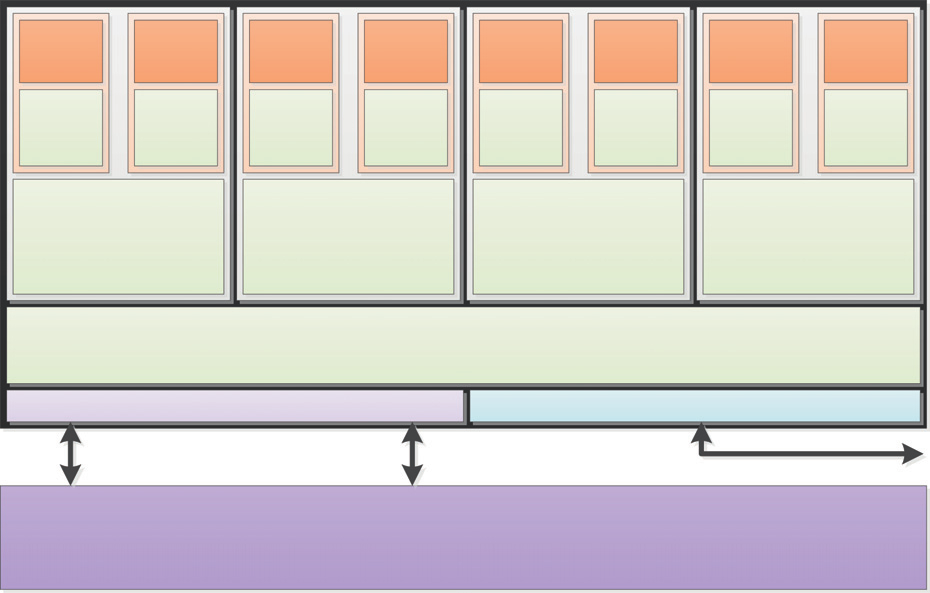
\includegraphics[width=\textwidth]{chapters/opencl/bulldozer.png}
  \end{center}
  \caption{Block diagram of hardware architecture of AMD FX--8150 CPU. Devices
    has 8 cores packed into 2--core logical modules sharing FPU unit, 2MiB of
    L2 data cache, instruction fetching/decoding units and branch predictor.}
  \label{fig:bulldozerarch}
\end{figure}
\todo{Replace \autoref{fig:bulldozerarch} with proper graphics.}
\subsection{OpenCL on NVIDIA GTX560Ti}
